\documentclass{standalone}

\usepackage{tikz}
\usetikzlibrary{shapes.geometric, arrows, calc}

\tikzstyle{class} = [rectangle, minimum width=3cm, minimum height=1cm, text centered, draw=black]

\usepackage{multicol}

\begin{document}
	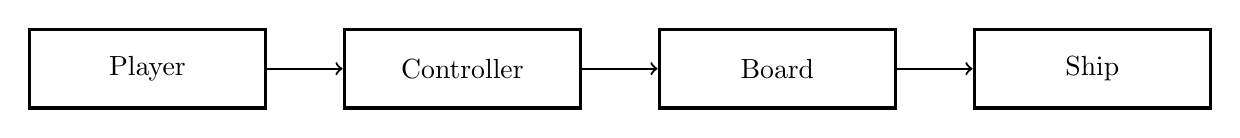
\begin{tikzpicture}
		\node[very thick] (player) [class] {Player};
		\node[very thick] (controller) [class] at ($(player) + (4, 0)$) {Controller};
		\node[very thick] (board) [class] at ($(controller) + (4, 0)$) {Board};
		\node[very thick] (ship) [class] at ($(board) + (4, 0)$) {Ship};
		
		\draw[->, thick] (player) -- (controller);
		\draw[->, thick] (controller) -- (board);
		\draw[->, thick] (board) -- (ship);
	\end{tikzpicture}
\end{document}